\documentclass[letterpaper]{article}
\usepackage{tikz-cd}
\usepackage{amsmath}
\usepackage{float}
\usepackage[spanish,activeacute]{babel}
\usepackage{amscd}
\usepackage{fancyhdr}
\usepackage{graphicx}
\usepackage{color}
\usepackage{transparent}
\usepackage{makeidx}
\usepackage{afterpage}
\usepackage{float}
\usepackage{amsmath, amsthm, amssymb, amsfonts, amssymb, amscd}
\usepackage{makeidx}
\usepackage{afterpage}
\usepackage{array}
\usepackage{pst-node}
\usepackage{hyperref}

\graphicspath{{./figs/}}
\newtheorem{teorema}{Teorema}[section]
\newtheorem{prop}[teorema]{Proposici\'on}
\newtheorem{cor}[teorema]{Corolario}
\newtheorem{lema}[teorema]{Lema}
\newtheorem{def.}{Definici\'on}[section]
\newtheorem{afir}{Afirmaci\'on}
\newtheorem{conjetura}{Conjetura}

\renewcommand{\figurename}{Figura}
\renewcommand{\indexname}{\'{I}ndice anal\'{\i}tico}

\newcommand{\zah}{\ensuremath{ \mathbb Z }}
\newcommand{\rac}{\ensuremath{ \mathbb Q }}
\newcommand{\nat}{\ensuremath{ \mathbb N }}
\newcommand{\prob}{\textbf{P}}
\newcommand{\esp}{\mathbb E}
\newcommand{\eje}{{\noindent \sc \textbf{Ejemplo. }}}
\newcommand{\obs}{{\noindent \sc \textbf{Observación. }}}
\newcommand{\dem}{{\noindent \sc Demostraci\'on. }}
\newcommand{\bg}{\ensuremath{\overline \Gamma}}
\newcommand{\ga}{\ensuremath{\Gamma}}
\newcommand{\fb}{\ensuremath{\overline F}}
\newcommand{\la}{\ensuremath{\Lambda}}
\newcommand{\om}{\ensuremath{\Omega}}
\newcommand{\sig}{\ensuremath{\Sigma}}
\newcommand{\bt}{\ensuremath{\overline T}}
\newcommand{\li}{\ensuremath{\mathbb{L}}}
\newcommand{\bs}{\ensuremath{\mathbb{S}^1}}
\newcommand{\co}{\ensuremath{\mathbb C }}
\newcommand{\con}{\ensuremath{\mathbb{C}^n}}
\newcommand{\hol}{\ensuremath{\mathcal{H}ol}}
\newcommand{\cp}{\ensuremath{\mathbb{CP}}}
\newcommand{\rp}{\ensuremath{\mathbb{RP}}}
\newcommand{\re}{\ensuremath{\mathbb R }}
\newcommand{\hc}{\ensuremath{\widehat{\mathbb C} }}
\newcommand{\pslz}{\ensuremath{\mathrm{PSL}(2,\mathbb Z) }}
\newcommand{\pslr}{\ensuremath{\mathrm{PSL}(2,\mathbb R) }}
\newcommand{\pslc}{\ensuremath{\mathrm{PSL}(2,\mathbb C) }}
\newcommand{\hd}{\ensuremath{\mathbb H^2}}
\newcommand{\slz}{\ensuremath{\mathrm{SL}(2,\mathbb Z) }}
\newcommand{\slr}{\ensuremath{\mathrm{SL}(2,\mathbb R) }}
\newcommand{\slc}{\ensuremath{\mathrm{SL}(2,\mathbb C) }}
\newcommand{\mdlr}{\ensuremath{\mathcal{M}}}
\newcommand{\lnb}{\ensuremath{\mathcal{O}}}
\newcommand{\Div}{\ensuremath{\mathrm{Div}}}
\newcommand{\ord}{\ensuremath{\mathrm{ord}}}
\newcommand{\hil}{\ensuremath{\mathcal H }}
\newcommand{\sph}{\ensuremath{\mathbb{S}}}
\newcommand{\nuc}{\ensuremath{\mathcal{N}}}
\newcommand{\cuat}{\ensuremath{\mathbb H}}
\newcommand{\modk}{\ensuremath{M_k(\Gamma)}}
\newcommand{\jac}{\ensuremath{\mathrm{J}(\sig)}}
\author{Carlos Eduardo Martínez Aguilar}
\date{\today}
\title{La Jacobiana de una superficie de Riemann y sus funciones theta.}
\hypersetup{
 pdfauthor={Carlos Eduardo artínez Aguilar},
 pdftitle={ La Jacobiana de una superficie de Riemann y sus funciones theta. },
 pdfkeywords={},
 pdflang={Esp}}
\begin{document}

\maketitle
\tableofcontents


\section{Introducción}
\noindent Describiremos la variedad Jacobiana de una superficie de Riemann compacta \(\sig\) y la relación entre su geometría y las propiedades de las funciones en la superficie. Describiremos el teorema de Riemann y Abel sobre la construcción e interpretación de la variedad Jacobiana de \(\sig\), denotada por \(\mathrm{J}(\sig)\) y su \emph{divisor theta} \(\theta(\sig)\). Veremos como las singularidades de dicho divisor theta codifican la información de ``El problema de Riemann-Roch'' para \(\sig\). Veremos el resultado clásico de Riemann, así como resultados más recientes como los de Andreotti-Mayer, Mumford y Kempf.
\subsection{Divisores y el grupo de Picard}
\begin{def.}
  Un  divisor en una variedad \(X\) es una combinación lineal formal
  \[
    D=\sum a_{i}Y_{i}\quad a_{i}\in\zah,\,Y_{i}\subset X \text{ hipersuperficie irreducible.}
  \]
\noindent Más aún, diremos que \(D\) es efectivo si \(a_{i}>0\). Naturalmente hablamos del grupo de divisores, el cual es el grupo libre generado por las hipersuperficies irreducibles en \(X\), y éste lo denotamos como \(\Div(X)\).
\end{def.}
\obs Si \(Y\subset X\) es una hipersuperficie y \(x\in Y\). Entonces \(Y\) define un germen irreducible en \(x\), el cual denotamos por \(g\in\mathcal{O}_{X,x}\), es decir, localmente cerca de \(x\), existe una vecindad \(U_{x}\), tal que
\[
  Y\cap U_{x}=V(g):=\{x\in U_{x}\,:\,g(x)=0\}.
\]
\noindent Por lo tanto si \(f\) es una función meromorfa en una vecindad de \(x\), el orden de \(f\) en \(x\) es el entero \(\ord_{x}(f)\in\zah\) tal que se cumple la igualdad
\[
  f=g^{\ord(f)_{x}}h\quad\text{donde }h\in\mathcal{O}^{*}_{X,x}=\{\phi\in\mathcal{O}_{X,x}\,:\,\phi(x)\neq0\}.
\]
\noindent Donde \(\ord_{x}(f)\) es independiente de \(g\), esto es claro de la irreducibilidad de \(g\). Si \(Y\) es irreducible, entonces definimos
\(\ord_{Y}(f):=\ord_{x}(f)\) con \(x\in Y\) cualquiera. Notamos que el orden es una función que satisface
\[
  \ord_{Y}(f_{1}f_{2})=\ord_{Y}(f_{1})+\ord_{Y}(f_{2}).
\]
Denotaremos por \(K(X)\) al conjunto de funciones meromorfas en \(X\).
\begin{def.}
  Sea \(f\in K(X)\), entonces asociaremos a \(f\) el siguiente divisor
  \[
    (f):=\sum_{Y}\ord_{Y}(f)Y=\sum_{\ord_{Y}(f)>0}\ord_{Y}(f)Y-\sum_{\ord_{Y}(f)<0}\ord_{Y}(f)Y=:Z(f)-P(f).
  \]
  \noindent Donde sumamos sobre todas las hipersuperficies irreducibles, llamaremos al los divisores \(Z(f)\) y \(P(f)\) \emph{el divisor cero} y \emph{el divisor de polos respectivamente}, ambos son divisores efectivos. Si \(D\in\Div(X)\) es tal que \(D=(f)\) para \(f\in K(X)\), diremos que \(D\) es un divisor \emph{principal}.
\end{def.}
Denotaremos por  \(\mathcal{K}_{X}\) al germen de funciones meromorfas, entonces claramente \(\mathcal{O}_{X}\subset\mathcal{K}_{X}\). Así generalizaremos la definición anterior para ahora poder definir divisores para secciones de haces de líneas
\begin{prop}
  Existe el siguiente isomorfismo natural
  \[
    H^{0}(X,\mathcal{K}^{*}_{X}/\mathcal{O}^{*}_{X})\cong\Div(X)\quad\text{donde }
    H^{0}(X,\mathcal{K}^{*}_{X}/\mathcal{O}^{*}_{X}):=\{s:X\rightarrow\mathcal{K}^{*}_{X}/\mathcal{O}^{*}_{X}\}
  \]
\end{prop}
\dem El isomorfismo consiste de definir para cada \(s\in H^{0}(X,\mathcal{K}^{*}_{X}/\mathcal{O}^{*}_{X})\) un divisor, para esto notamos que localmente \(s\) está dada por una función meromorfa. Las condiciones de cociclo aseguran que los órdenes de estas funciones son independientes de los representates de los cociclos, así
\[
  s\mapsto (s)=\sum_{Y}\ord_{Y}(s)Y\in\Div(X),
\]
\noindent está bien definido. Ahora si \(D\in\Div(X)\), entonces
\[
  D=\sum^{n}_{i=1}a_{i}Y_{i}\in\Div(X),
\]
\noindent ahora existe una cubierta abierta tal que
\[
  X=\bigcup_{i\in I}U_{i}\quad Y_{i}\cap U_{j}=V(g_{i,j}),\,g_{i,j}\in\mathcal{O}(U_{j})
\]
Es claro que las funciones
\[
  f_{j}:=\prod^{n}_{i=1}g^{a_{i}}_{i,j}\in\mathcal{K}^{*}_{X}(U_{j})
\]
\noindent definen una sección \(s\in H^{0}(X,\mathcal{K}^{*}_{X}/\mathcal{O}^{*}_{X})\).\qed

\obs En geometría algebraica no siempre existe este isomorfismo, por lo tanto hay una distinción entre estos dos tipos de divisores, al grupo \(H^{0}(X,\mathcal{K}^{*}_{X}/\mathcal{O}^{*}_{X})\) se es conoce como los divisores \emph{Cartier}, y a los divisores \(\Div(X)\) se les conoce somo divisores de \emph{Weil}.
\begin{def.}
  Definimos el grado de un divisor como el morfismo de grupos abelianos \(\deg:Div(X)\rightarrow\zah\)
  \[
    D=\sum_{i}a_{i}Y_{i}\,\mapsto\,\deg(D)=\sum_{i}a_{i}.
  \]
 Un divisor es \emph{efectivo} si \(D\geq0\), es decir \(a_{i}\geq0\) para toda \(i\).
\end{def.}

\begin{def.}
  El grupo de Picard de una variedad holomorfa \(X\), se define como el grupo de las clases de isomorfismos de haces de líneas en \(X\), el cual denotaremos por \(\mathrm{Pic}(X)\), donde el producto e inverso se definen por medio del producto tensorial y dualizacion respectivamente,  es decir
  \[
    \lnb_{1}+\lnb_{2}:=\lnb_{1}\otimes\lnb_{2}\hspace{0.2cm}\forall\,\{\lnb_{1},\lnb_{2}\}\subset\mathrm{Pic}(X)\quad\lnb^{-1}:=\lnb^{*}\hspace{0.2cm}\forall\,\lnb\in\mathrm{Pic}(X).
  \]
  \noindent Además el neutro es el \emph{haz de líneas trivial}
  \[
    \mathcal{O}(0):=\co\times X.
  \]
\end{def.}
\obs Existe un isomorfismo natural \(\mathrm{Pic}(X)\cong H^{1}(X,\mathcal{O}^{*}_{X})\), dado por las condiciones de cociclo, esto es ciero para la cohomología de Cech.
\begin{prop}
  Existe un morfismo de grupos natural
  \[
    \Div(X)\rightarrow\mathrm{Pic}(X)\quad D\mapsto \lnb(D).
  \]
\end{prop}
\dem Dado un divisor \(D=\sum a_{i}Y_{i}\in\Div(X)\), le corresponde una sección \(s\in H^{0}(X,\mathcal{K}^{*}_{X}/\mathcal{O}^{*}_{X})\), de tal manera que en una cubiertaa abierta se tiene que
\[
  X=\bigcup_{i\in I}U_{i}\quad s|_{U_{i}}=f_{i}\in\mathcal{K}^{*}(U_{i}),
\]
\noindent entonces definimos \(\lnb(D)\in\mathrm{Pic}(X)\) como el haz de líneas definido por las funciones de transición (cociclos)
\[
  \psi_{i,j}:=\frac{f_{i}}{f_{j}}\in H^{1}(U_{i}\cap U_{j},\mathcal{O}^{*}_{X}),
\]
\noindent entonces como claramente se cumplen las condiciones de cociclo, por lo que representan un elemento de \(\mathrm{Pic}(X)\). Ahora veamos que en efecto es un homomorfismo de grupos, supongamos \(\{D_{1},D_{2}\}\subset\Div(X)\) y \(\{f_{i}\},\{g_{i}\}\) son los correspondientes cociclos de \(\lnb(D_{1})\) y \(\lnb(D_{2})\) respectivamente, entonces los cociclos de \(D_{1}+D_{2}\) corresponden a \(\{f_{i}g_{i}\}\) (es posible que se necesita pasar por un refinamiento de las cubiertas). Por lo tanto es claro que \(\lnb(D_{1}+D_{2})=\lnb(D_{1})\otimes\lnb(D_{2})\). \qed
\subsection{Superficies de Riemann compactas y el teorema de Riemann-Roch.}
\noindent Sea \(\sig\) una superficie de Riemann compacta de género \(g\) y sea \(D=p_{1}+\cdots+p_{d}\), donde \(p_{i}\in\sig\) un divisor efectivo de grado \(d\) en \(\sig\). Entonces como hemos visto, existe un haz de líneas asociado, \(\lnb(D)\) en \(\sig\), con una sección \(\sigma\in H^{0}(X,\lnb(D))\) tal que \((\sigma)=D\). Definimos el espacio de funciones meromorfas en \(\sig\) \emph{dominadas} por \(D\) como
\[
  L(D)=\{f\in\mathcal{K}_{\sig}\,:\,(f)+D\geq0\}.
\]
Además, notamos que el morfismo
\[
  H^{0}(X,\lnb(D))\rightarrow L(D)   \quad \tau\mapsto\frac{\tau}{\sigma},
\]
\noindent es un isomorfismo (\(Z-P\)).

\emph{El problema de ``Riemann-Roch''} es calcular el número
\[
  h^{0}(D)=\dim_{\co}H^{0}(\lnb(D)),
\]
es decir, contar el número de secciones independientes de un haz de líneas. La respuesta, diemuestra que este número es finito y como es de esperarse se encuentra en el resultado
\begin{teorema}[Riemann-Roch]
  Sea \(\sig\) una superficie de Riemann de género \(g\) y sea \(K\) el divisor cero de una 1-forma en \(\sig\), si denotamos por \(\lnb_{K}=\lnb(K)\) a su haz de líneas canónico, entonces para todo divisor \(D\) de grado \(d\) en \(\sig\),
  \[
    h^{0}(D)-h^{0}(K-D)=1-g+d.
  \]
  Más aún, si \(D=(\sigma)\), con \(\sigma\in H^{0}(\sig,\lnb_{D}) \), entonces \(\sigma\) nos da un isomorfismo
  \[
    H^{0}(\sig,\lnb_{K-D})\rightarrow L(-D)
  \]

\end{teorema}
Sin embargo, esto no resuelve el problema de calcular \(h^{0}(D)\) ya que es simplemente una relación entre éste y \(h^{0}(K-D)\). Si se toma \(D=0\) o \(D=K\), se obtiene \(h^{0}(K)=g\) y \(\deg(K)=2g-2\) respectivamente. Más aún, como los divisores de funciones meromorfas tienen grado cero, \((f)+D\geq0\) es imposible para \(D\) de grados negativos, lo que significa que \(d<0\) implica \(h^{0}(D)=0\). Similarmente \(d>2g-2\) implica \(h^{0}(D)=1-g+d\). Por lo que el problema de Riemann-Roch es especialmente interesante para divisores con grado \(0<d<2g-2\) y la variedad Jacobiana y la función theta de Riemann son herramientas fundamentales para esto.
\section{La Jacobiana de \(\sig\)}
\noindent Comenzamos recordando que si \(\{\omega_{1},\dots,\omega_{g}\},\,g\geq2\) es una base de 1-formas diferenciales para el espacio \(H^{0}(\sig,\lnb_{K})\), y \(p\in\sig\) es un punto cualquiera, el vector \((\omega_{1}(p),\dots,\omega_{g}(p))\in\co^{g}\) está bien definido independientemente de la base salvo un múltiplo escalar y claramente nunca es nulo, es decir, define un mapeo
\[
  \phi_{K}:\sig\rightarrow\cp^{g-1}\quad p\mapsto[\omega_{1}(p):\dots:\omega_{g}(p)],
\]
\noindent el cual es un encaje, de \(\sig\) en una curva \(\ga\) de grado \(2g-2\) que genera \(\cp^{g-1}\). Excepto en el caso de que \(\sig\) sea una superficie \emph{``hiperelíptica''}, esto quiere decir que \(\sig\) admite una  1-forma meromorfa con dos polos, en cuyo caso \(\phi_{K}\) es un mapeo dos a uno sobre una curva \(\ga\) de grado \(g-1\) isomorfa a \(\cp^{1}\).
Como \(\phi_{K}\) se puede definir independientemente de la base, tenemos
\[
  \phi_{K}:\sig\rightarrow\cp(H^{0}(\sig,\lnb_{K}))\quad\phi_{K}(p)=\{\omega\,:\,\omega(p)=0\}=\ker(ev_{p}),
\]
\noindent donde tomamos el punto de vista dual y a cada 1-forma \(\omega\) la identificamos con una funcional lineal y su hiperplano generado corta con la curva encajada \(\ga=\phi_{k}(\sig)\) en el divisor \(K=(\omega)=Z(\omega)\).
Ahora sean \(\{\alpha_{1},\dots,\alpha_{g},\beta_{1},\dots,\beta_{g}\}\) una base simpléctica de la homología entera, es decir una base \(H_{1}(\sig,\zah)\) como se ve en la figura.
\begin{figure}[htb]
\begin{center}
\includegraphics[height=5cm,width=10cm]{dibujo-2.pdf}
  \caption{Superficie con ciclos generadores.}
  \label{fig:base-simp}
\end{center}
\end{figure}

Entonces existe una única base \(\{\omega_{1},\dots,\omega_{g}\}\) de \(H^{0}(\sig,\lnb_{K})\) tal que
\[
  \Big(\int_{\alpha_{i}}\omega_{j}\Big)=(\delta_{i,j})=\mathrm{I}_{g}.
\]
Además definimos la siguiente matriz
\[
  \tau=(\tau_{i,j})=\Big(\int_{\beta_{i}}\omega_{j}\Big),
\]
la cual es una matriz simétrica compleja de \(g\times g\) con parte imaginaria positiva definida. Si \(\Lambda\) es la latiz entera en \(\co^{g}\) generada por las \(2g\) columnas de la matriz \(\mathrm{I}\tau\), entonces
\begin{def.}
  La variedad Jacobiana de \(\sig\) es el toro compacto complejo
  \[
    \mathrm{J}(\sig)=\co^{g}/\Lambda.
  \]
\end{def.}
\obs Intrinsecamente esto significa que
\[
  \mathrm{J}(\sig)=H^{0}(\sig,\lnb_{K})^{*}/H_{1}(\sig,\zah)
\]
\subsection{El mapeo de Abel}
\noindent Para cada punto base \(p_{0}\in\sig\), existe \(u_{0}:\sig\rightarrow\mathrm{J}(\sig)\) definida por
\[
  u_{0}(p)=\Big(\int^{p}_{p_{0}}\omega_{1},\dots,\int^{p}_{p_{0}}\omega_{g}\Big)\mod\Lambda.
\]
Esta es una herramienta para usar \(\mathrm{J}(\sig)\) para estudiar \(\sig\) y viceversa.\\
Si \hbox{\(\sig^{d}=\sig\times\cdots\times\sig\)}, entonces definimos
\[
  \sig_{d}=\sig^{d}/S_{d}\quad S_{d}=\mathrm{Sym}(I_{d}=\{1,\dots,d\})=\{\sigma:I_{d}\rightarrow I_{d}\,|\,\sigma\text{ biyectiva}\},
\]
\noindent donde la acción de \(S_{d}\) esta dada por las permutaciones de las coordenadas
\[
  \sigma(z_{1},\dots,z_{j},\dots,z_{d})=(z_{\sigma(1)},\dots,z_{\sigma(j)},\dots,z_{\sigma(d)}).
\]
\noindent Este espacio es el espacio natural de parámetros para los divisores efectivos de grado \(d\). Entonces el mapeo de Abel se define como la extensión natural de \(u_{0}\) a \(\sig_{d}\), es decir
\[
  U_{0}(p_{1},\dots,p_{d})=\sum^{d}_{j=1}u_{0}(p_{j})= \sum^{d}_{j=1}\Big(\int^{p_{j}}_{p_{0}}\omega_{1},\dots,\int^{p_{j}}_{p_{0}}\omega_{g}\Big)\mod\Lambda.
\]
\obs Tanto \(\sig_{d}\) como \(\sig^{d}\) son varidades compactas complejas y holomorfas de dimensión \(d\) y como el mapeo de Abel es holomorfo en coordenadas, entonces es holomorfo globalmente, sin embargo para algunos cálculos se usará \(\sig^{d}\) a pesar de que \(\sig_{d}\) se relaciona de manera más directa con los divisores. En este sentido a cada punto en \([D]=[p_{1},\cdots,p_{d}]\in\sig_{d}\), le corresponde un único divisor de grado \(d\) en \(\sig\), simplemente asociamos a \([D]\) la suma \(D=p_{1}+\cdots+p_{d}\) la cual queda unicamente determinada pues los puntos de \(\sig_{d}\) son identificados bajo permutaciones. Por lo que denotaremos a los puntos de \(\sig_{d}\) como divisores \(D=p_{1}+\cdots+p_{d}\), así es claro que \(u_{0}\) es el mapeo de Abel de divisores de grado uno mientras que \(U_{0}\) es el caso general.
\subsubsection{La derivada del mapeo de Abel}
Primero notamos que para cada \(u\in\jac\) el espacio tangente proyectivizado es  naturalmente isomorfo a
\[
  \cp(T_{u}\jac)\cong\cp(T_{0}\jac)\cong\cp(H^{0}(\sig,\lnb_{K})^{*}).
\]
\noindent Luego, para cada \(p\in\sig\) la imagen del espacio \(u_{0*}(T_{p}\sig)\), es simplemente la imagen de las derivadas de los componentes de \(u_{0}\), las cuales por el teorema fundamental del cálculo son \((\omega_{1}(p),\dots,\omega_{g}(p))=\phi_{K}(p)\), la imágen canónica de \(p\) en \(\cp(H^{0}(\sig,\lnb_{K})^{*})\). Por lo tanto la derivada del mapeo del mapeo de Abel es el mapeo canónico. En el caso del mapeo de Abel en \(\sig_{d}\), consideramos un divisor \(D=p_{1}+\dots+ p_{d}\in\sig_{d}\), la imagen de \(U_{0*}(T_{D}\sig_{d})\) en \(\cp(T_{0}\jac)=\cp^{g-1}\) es el espacio generado por
\[
  \{\phi_{K}(p_{1}),\dots,\phi_{K}(p_{d})\}.
\]
\noindent En particular \(U_{0*}\) tiene rango \(d\) en \(D\) si y sólo dichos puntos son linealmente independientes en \(\cp^{g-1}\) si y sólo si se encuentran contenidos en \(g-d\) hiperplanos independientes, sí y sólo si los puntos son distintos y \(h^{0}(K-D)=g-d\).
\subsection{La función theta de Riemann}
\noindent Los mapeos de Abel son mapeos \(\sig\rightarrow\jac\), en este sentido, es natural preguntarse por mapeos ``fuera'' o que ``salgan'' de \(\jac\), para esto la función theta de Riemann es una función natural. Supongamos que fijamos una base simpléctica para la homología y su base asociada en \(H^{0}(\sig,\lnb_{K})\), la función theta depende de esta elección unicamente por traslaciones en \(\jac\).
\begin{def.}
  Sea \(\tau\) la matriz previamente definida, con \(\tau=\tau^{t}\) y \(Im(\tau)\) positiva definida, entonces definimos \(\theta_{\sig}:\co^{g}\rightarrow\co\)
  \[
    \theta_{\sig}(z)=\sum_{n\in\zah^{g}}\exp(i\pi((n^{t}\tau n)+2n^{t}z)).
  \]
  \noindent Esta es una función meromorfa, cuyo divisor cero es periódico con respecto a la latiz \(\Lambda\) y por lo tanto define un divisor \(\theta(\sig)\subset\jac\)
\end{def.}
Ahora, si recordamos el mapeo de Piccard \(Div(\sig)\rightarrow\mathrm{Pic}(\sig)\), este claramente es suprayectivo pues podemos tomar el divisor generado de los cociclos locales, esto quiere decir que
\[
  \mathrm{Pic}(\sig)\cong Div(\sig)/H\quad H=\{\lnb_{D}\cong\sig\times\co\iff\deg(D)=0\iff D=(f),\,f\in\mathcal{K}^{*}_{\sig}\}.
\]
Entonces, como discutimos previamente \(\cp(H^{0}(X,\lnb_{D}))\cong |D|\subset\sig_{d}\) donde \(|D|\) es el conjunto de clases de divisores de la forma \(D+(f)\). Por lo tanto el problema de Riemann-Roch es el problema de entender la dimensión de las fibras del mapeo de Piccard.
\[
  v_{k}:\sig_{d}\rightarrow\mathrm{Pic}^{k}(\sig)\quad D\mapsto\lnb(D).
\]
\noindent Donde, \(\mathrm{Pic}^{k}(\sig)=\{\text{Clases de isomorfismo de haces de grado }k\}\)
\begin{teorema}[Abel]
  Existe un isomorfismo natural entre \(\mathrm{Pic}^{0}(\sig)\) y \(\jac\) tal que bajo cualquier elección de punto base \(p_{0}\in\sig\), los mapeos de Abel y Piccard \(U_{0}:\sig_{d}\rightarrow\jac\) y \(v_{0}:\sig_{d}\rightarrow\mathrm{Pic}^{0}(\sig)\) respectivamente, donde \(v_{0}(D)=\lnb(D-d*p_{0})\)  hacen conmutar el diagrama
  \begin{equation}
    \begin{tikzcd}
    \sig_{d} \arrow{r}{u_{0}} \arrow[swap]{dr}{v_{0}} & \jac \arrow{d}{\cong} \\
                                                & \mathrm{Pic}^{0}(\sig)
    \end{tikzcd}
\end{equation}
\end{teorema}
\noindent Es decir que la variedad de Piccard \(\mathrm{Pic}^{0}(\sig)\) no solo es un grupo sino que hereda la estructura de toro complejo de \(\jac\), lo cual hace al mapeo de Piccard holomorfo.
\begin{teorema}[Riemann]
  Dada una elección de las bases de homología simplecticas enteras y de la matriz \(\tau\) y por ende de la función \(\theta_{\sig}\), existe una raiz cuadrada \(\kappa\in\mathrm{Pic}^{g-1}(\sig)\) del haz de líneas canónico \(K\in\mathrm{Pic}^{2g-2}(\sig)\), tal que el isomorfismo
  \[
    \mathrm{Pic}^{g-1}(\sig)\cong\mathrm{Pic}^{0}(\sig)=\jac,
  \]
  dado por la traslación por \(\kappa\) mapea \(W_{g-1}=v_{g-1}(\sig_{d})\) isomorficamente en \(\theta(\sig)\).
\end{teorema}
\begin{cor}[Lema intrínseco de Riemann]
  Sea \(D\in\sig_{g}\) un divisor efectivo, defina el mapedo de Piccard modificado como
  \[
    \sigma_{D}:\sig\to\mathrm{Pic}(\sig)\quad p\mapsto\sigma_{D}(p)=\lnb(D-p).
  \]
  Entonces se tiene que \(h^{0}(D)>1\) y \(\sigma_{D}(\sig)\subset W_{g-1}\) o \(h^{0}(D)=1\) y el divisor de intersección es \(\sigma_{D}(\sig) W_{g-1}=D\).
  \end{cor}
\end{document}
